\documentclass[10pt,a4paper]{article}
\usepackage[margin=1.6cm]{geometry}
\usepackage[latin1]{inputenc}
\usepackage{amsmath}
\usepackage{amsfonts}
\usepackage{amssymb}
\usepackage{multirow}
\usepackage{graphicx}
\usepackage{subcaption}

\setlength{\parskip}{5pt}
\setlength{\parindent}{0pt}

\author{Hector Dearman \and Paul Rowe-White \and Kritaphat Songsriin \and Simon Stuckemann}
\title{Machine Learning CBC: Neural Networks}
\begin{document}
\maketitle

\section{Implementation Details}
\subsection{Cross-Validation}
summary of implementation details, e.g. how we performed cross-validation

\subsection{Classification}
how we classified each example based on the 6 outputs, anything we think is important
flow chart

\subsection{Pre-processing and Post-processing}

\section{Evaluation Process}

\subsection{Finding Optimal Parameters (1)}
We assumed the parameters to be independent.
This is not a good assumption since the parameters are not necessarily independent however it is necessary to make the problem of optimising the parameters tractable.
We first set out each parameter we would have to optimise ???

To optimise a parameter we took the first fold of the data then for each value of the parameter we where trying we preformed three fold cross validation on that fold recording the average sum of the performance measure over each example in the validation set.
After doing this for each parameter value we selected the value with best performance measure

For most of the parameters it was possible to do a exhaustive (grid) search (after fixing a reasonable range and step size) however for the topology of the network, the number of layers and the number of nodes within each layer, it still proved impractical to try every combination.
We did two things to make optimising the topology possible in the time we had, we considered only topologies where every layer had the same number of nodes and we used a two layer search, first finding the best number of nodes to the nearest ten then we have a second search of the ten values on either side of the best result of the larger step\footnote{This will only be the true optimum value if the performance measure given the number of nodes is convex however so long as the larger step is smaller than large fluctuations in the performance measure this should do reasonably well.}.

???
- How we obtained the optimal parameters, topology
How should we be optimising parameters (not in the first fold only)
different topologies and parameters we experimented with

\subsection{Performance measure (1)}
Initially we used the classification error as a performance measure. 
This worked when we were building the six-output network however when we were building the one-output network this was difficult since you would like to train and optimise each individual network without having to guess whether the particular output it gave would be enough to classify an example.
We could have considered outputs less than 0.5 to be a negative classification however we would really like penalise or reward an output based on how right or how wrong it was.
Concretely if an example is labelled 0 and we predict 0.6 it's less bad (and our performance measure should give a better score) then if we predict 1.0. 

To do this we used the following logistic cost function:

\[
    Cost(p, y)= 
\begin{cases}
    -\log{p}& \text{if } y = 1\\
    -\log{(1 - p)}              & \text{if } y = 0
\end{cases}
\]

Where $p$ is the prediction for an example and $y$ is it's true label.
We take the sum of this cost function over every example in the validation set as our performance measure 
This new function gave very similar results to the previous measure on the six-output networks so we where confident it was not completely wrong.

\begin{figure}[!ht]
     \centering
     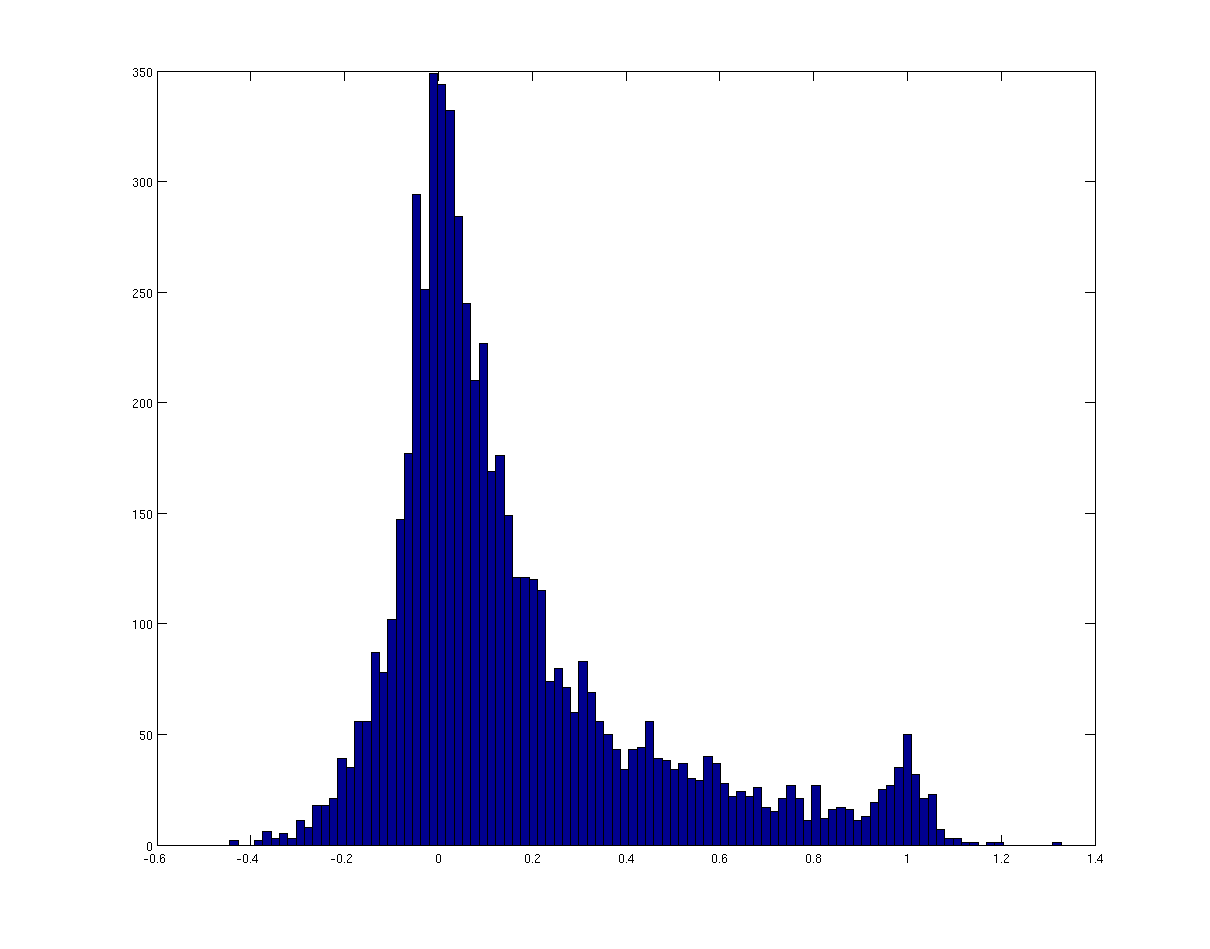
\includegraphics[width=\textwidth]{../../images/clean_hist.png}
     \caption{Histogram of Neural Network output}
     \label{fig:tree2}
\end{figure}


\subsection{Avoiding Overfitting (2)}
We used a few techniques to avoid overfitting the first and most important 

\subsection{How should we optimise parameters (3)}
performance measure we used why we preferred it over other ones

\section{Results (3)}

any difference between the average classification performance of the two types, both clean and noisy data. Discuss advantages and disadvantages

Commented results on average confusion matrices for both types of network and both clean and noisy with 
	- avg. classification rate
	- recall rate, precision rate, and F1 per class

figures of the average performance per fold for both types and nosiy/clean; discussion

\begin{figure}[!ht]
	\centering
	\begin{subfigure}[b]{0.7\textwidth}
		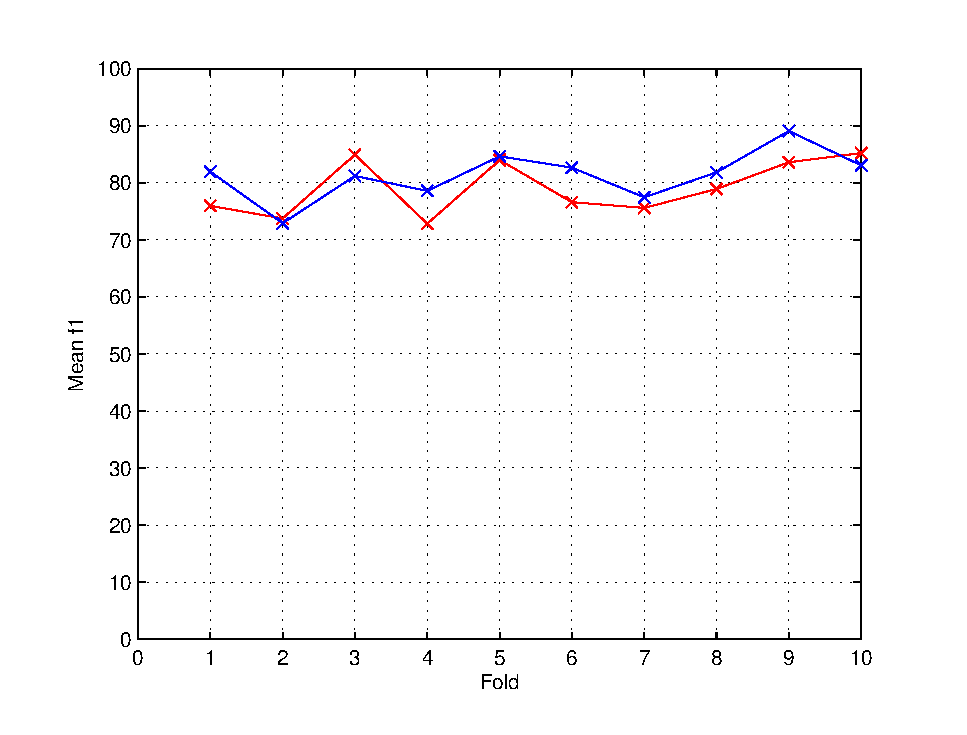
\includegraphics[width=\textwidth]{images/clean_fold_f1_plot.eps}
     	\caption{Average value of F1 measure for all 6 emotions against folds for clean data}
     	\label{fig:avgF1Clean}
    \end{subfigure}
	\begin{subfigure}[b]{0.7\textwidth}
		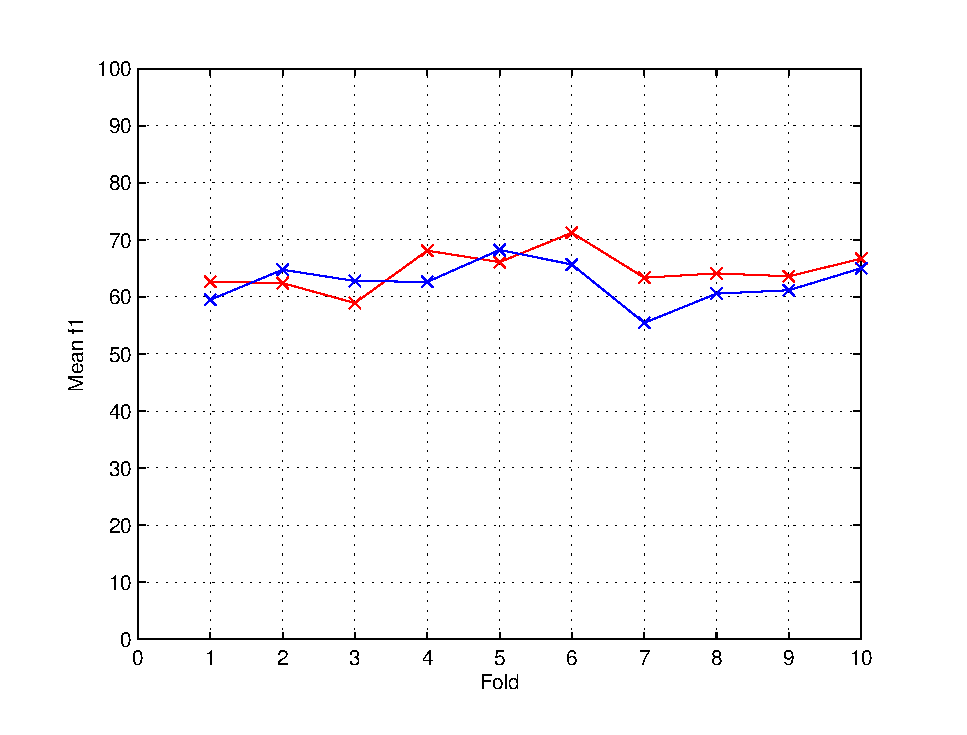
\includegraphics[width=\textwidth]{images/noisy_fold_f1_plot.eps}
     	\caption{Average value of F1 measure for all 6 emotions against folds for noisy data}
     	\label{fig:avgF1Noisy}
    \end{subfigure}
    \caption{Red: Six Output NN, Blue: Single Output NNs}
    \label{fig:avgF1}
\end{figure}

\begin{table}[!ht]
\centering
\begin{tabular}{|l|c|c|c|c|c|c|c|}
	\cline{3-8}
	\multicolumn{2}{c}{}& \multicolumn{6}{ |c| }{Predicted class}\\
	\cline{3-8}
	\multicolumn{2}{c|}{} & 1 & 2 & 3 & 4 & 5 & 6\\ \cline{1-8}
	\multirow{6}{*}{Actual class}& 1 & 9.1 & 1.5 & 0.5 & 0.3 & 1.6 & 0.1 \\ \cline{2-8}
	& 2 & 1.1 & 16.1 & 0.4 & 0.4 & 1.6 & 0.2\\ \cline{2-8}
	& 3 & 0.4 & 0.3 & 9.5 & 0.1 & 0.4 & 1.1 \\ \cline{2-8}
	& 4 & 0.1 & 0.6 & 0.3 & 20.1 & 0.2 & 0.2 \\ \cline{2-8}
	& 5 & 1.2 & 2.3 & 0.5 & 0.5 & 8.4 & 0.3 \\ \cline{2-8}
	& 6 & 0.1 & 0.2 & 0.7 & 0.6 & 0.4 & 18.6\\ \hline
\end{tabular}
\caption{Confusion Matrix of Six Output NN - Clean Data}
\label{tab:sixOutputCleanConfusion}
\end{table}

\begin{table}[!ht]
\centering
\begin{tabular}{|l|c|c|c|c|c|c|c|}
	\cline{3-8}
	\multicolumn{2}{c}{}& \multicolumn{6}{ |c| }{Predicted class}\\
	\cline{3-8}
	\multicolumn{2}{c|}{} & 1 & 2 & 3 & 4 & 5 & 6\\ \cline{1-8}
	\multirow{6}{*}{Actual class}& 1 & 1.1 & 1.5 & 2.4 & 0.9 & 2.1 & 0.8 \\ \cline{2-8}
	& 2 & 0.2 & 15.2 & 1.6 & 0.4 & 0.8 & 0.5\\ \cline{2-8}
	& 3 & 0.3 & 1.4 & 13.7 & 1.1 & 0.5 & 1.7 \\ \cline{2-8}
	& 4 & 0.2 & 0.6 & 0.6 & 18.4 & 0.4 & 0.6 \\ \cline{2-8}
	& 5 & 0.6 & 0.8 & 1.4 & 0.3 & 6.8 & 1.1 \\ \cline{2-8}
	& 6 & 0.1 & 0.3 & 1.4 & 1.1 & 0.8 & 18.3\\ \hline
\end{tabular}
\caption{Confusion Matrix of Six Output NN - Noisy Data}
\label{tab:sixOutputNoisyConfusion}
\end{table}

\begin{table}[!ht]
\centering
\begin{tabular}{|l|c|c|c|c|c|c|c|}
	\cline{3-8}
	\multicolumn{2}{c}{}& \multicolumn{6}{ |c| }{Predicted class}\\
	\cline{3-8}
	\multicolumn{2}{c|}{} & 1 & 2 & 3 & 4 & 5 & 6\\ \cline{1-8}
	\multirow{6}{*}{Actual class}& 1 & 9.4 & 1.3 & 0.6 & 0.6 & 1.1 & 0.1 \\ \cline{2-8}
	& 2 & 1.2 & 15.9 & 0.3 & 0.7 & 1.6 & 0.1\\ \cline{2-8}
	& 3 & 0.7 & 0.2 & 9.6 & 0 & 0.4 & 0.9 \\ \cline{2-8}
	& 4 & 0.1 & 0.7 & 0 & 20.2 & 0.3 & 0.2 \\ \cline{2-8}
	& 5 & 0.8 & 1.7 & 0.5 & 0.4 & 9.6 & 0.2 \\ \cline{2-8}
	& 6 & 0 & 0.4 & 0.9 & 0.4 & 0.3 & 18.6\\ \hline
\end{tabular}
\caption{Confusion Matrix of Six Single Output NNs - Clean Data}
\label{tab:sixSingleOutputsCleanConfusion}
\end{table}

\begin{table}[!ht]
\centering
\begin{tabular}{|l|c|c|c|c|c|c|c|}
	\cline{3-8}
	\multicolumn{2}{c}{}& \multicolumn{6}{ |c| }{Predicted class}\\
	\cline{3-8}
	\multicolumn{2}{c|}{} & 1 & 2 & 3 & 4 & 5 & 6\\ \cline{1-8}
	\multirow{6}{*}{Actual class}& 1 & 1.6 & 1.7 & 2 & 1.1 & 2.1 & 0.3 \\ \cline{2-8}
	& 2 & 0.2 & 15.6 & 1.4 & 0.7 & 0.6 & 0.2\\ \cline{2-8}
	& 3 & 0.5 & 2 & 12 & 1 & 1 & 2.2 \\ \cline{2-8}
	& 4 & 0.1 & 0.7 & 1 & 17.9 & 0.5 & 0.6 \\ \cline{2-8}
	& 5 & 1.3 & 1 & 1.4 & 0.5 & 5.6 & 1.2 \\ \cline{2-8}
	& 6 & 0.2 & 0.6 & 1.5 & 0.5 & 1 & 18.2\\ \hline
\end{tabular}
\caption{Confusion Matrix of Six Single Output NNs - Noisy Data}
\label{tab:sixSingleOutputsNoisyConfusion}
\end{table}

\begin{table}[!ht]
\centering
\begin{tabular}{|l|c|c|c|}
	\cline{3-3}
	\multicolumn{2}{c|}{} & Average Classification Rate \\ \cline{1-3}
	\multirow{2}{*}{Network}& Six Output (Clean) & 0.8180  \\ \cline{2-3}  
	& Six Output (Noisy) & 0.7350  \\ \cline{2-3} 
		& Single Outputs (Clean) & 0.8330 \\ \cline{2-3} 
	& Single Outputs (Noisy) & 0.7090 \\ \hline

\end{tabular}
\caption{Average Classification Rate}
\label{tab:avgClassificationRate}
\end{table}

\begin{table}[!ht]
\centering
\begin{tabular}{|l|c|c|c|c|c|c|c|}
	\cline{3-8}
	\multicolumn{2}{c}{}& \multicolumn{6}{ |c| }{Class}\\
	\cline{3-8}
	\multicolumn{2}{c|}{} & 1 & 2 & 3 & 4 & 5 & 6\\ \cline{1-8}
	\multirow{2}{*}{Network}& Six Output (Clean) & 69.4656 & 81.3131 & 80.5085 & 93.4884 & 63.6364 & 90.2913 \\ \cline{2-8}  
	& Six Output (Noisy) & 12.5 & 81.2834 & 73.2620 & 88.4615 & 61.8182 & 83.1818 \\ \cline{2-8} 
		& Single Outputs (Clean) & 71.7557 & 80.3030 & 81.3559 & 93.9535 & 72.7273 & 90.2913\\ \cline{2-8} 
	& Single Outputs (Noisy) & 18.1818 & 83.4225 & 64.1711 & 86.0577 & 50.9091 & 82.7273\\ \hline

\end{tabular}
\caption{Recall Per Class}
\label{tab:recallPerClass}
\end{table}

\begin{table}[!ht]
\centering
\begin{tabular}{|l|c|c|c|c|c|c|c|}
	\cline{3-8}
	\multicolumn{2}{c}{}& \multicolumn{6}{ |c| }{Class}\\
	\cline{3-8}
	\multicolumn{2}{c|}{} & 1 & 2 & 3 & 4 & 5 & 6\\ \cline{1-8}
	\multirow{2}{*}{Network}& Six Output (Clean) & 75.8333 & 76.6667 & 79.8319 & 91.3636 & 66.6667 & 90.07317 \\ \cline{2-8}  
	& Six Output (Noisy) & 44 & 76.7677 & 64.9289 & 82.8829 & 59.6491 & 79.5652 \\ \cline{2-8} 
		& Single Outputs (Clean) & 77.0492 & 78.7129 & 80.6723 & 90.5830 & 72.1805 & 92.5373\\ \cline{2-8} 
	& Single Outputs (Noisy) & 41.0256 & 72.2222 & 62.1762 & 82.4885 & 51.8519 & 80.1762\\ \hline

\end{tabular}
\caption{Precision Per Class}
\label{tab:precisionPerClass}
\end{table}

\begin{table}[!ht]
\centering
\begin{tabular}{|l|c|c|c|c|c|c|c|}
	\cline{3-8}
	\multicolumn{2}{c}{}& \multicolumn{6}{ |c| }{Class}\\
	\cline{3-8}
	\multicolumn{2}{c|}{} & 1 & 2 & 3 & 4 & 5 & 6\\ \cline{1-8}
	\multirow{2}{*}{Network}& Six Output (Clean) & 72.51 & 78.9216 & 80.1688 & 92.4138 & 65.1163 & 90.5109 \\ \cline{2-8}  
	& Six Output (Noisy) & 19.4690 & 78.9610 & 68.8442 & 85.5814 & 60.7143 & 81.3333 \\ \cline{2-8} 
		& Single Outputs (Clean) & 74.3083 & 79.5 & 81.0127 & 92.2374 & 72.4528 & 91.4005\\ \cline{2-8} 
	& Single Outputs (Noisy) & 25.1969 & 77.4194 & 63.1579 & 84.2353 & 51.3761 & 81.4318\\ \hline

\end{tabular}
\caption{F1 Measure Per Class}
\label{tab:f1MeasurenPerClass}
\end{table}

\end{document}
